\begin{defn}
  Uno spazio topologico $X$ localmente connesso per archi si dice \textsc{semilocalmente semplicemente connesso} se per ogni $x \in X$ esiste $U \subseteq X$ aperto con $x \in U$ t.c. l'inclusione $i:U \rightarrow X$ induce il morfismo banale $i_{\star}:\pi_1(U, x) \rightarrow \pi_1(X, x)$. Ovvero, per ogni $x \in X$ esiste un intorno $U$ di $x$ t.c. tutti i lacci basati in $x$ e contenuti in $U$ sono banali in $X$.
\end{defn}

Questa proprietà è verificata ad esempio se ogni punto ha un intorno semplicemente connesso (per esempio le varietà).

\begin{oss}
  Se $X$ ammette un rivestimento universale, allora è semilocalmente semplicemente connesso. Infatti, dato $x \in X$, ne possiamo prendere un intorno connesso per archi e ben rivestito $U$. Se $p:E \rightarrow X$ è il rivestimento universale e $V \subseteq p^{-1}(U)$ è un aperto con $p\restrict{V}:V \rightarrow U$ omeomorfismo,
  \begin{center}
    \begin{tikzcd}
      V \arrow[r, hook, "j"] \arrow[d, shift left, swap, "p\restrict{V}" right] & E \arrow[d, "p"]\\
      U \arrow[r, hook, "i"] \arrow[u, shift left, "s"] & X
    \end{tikzcd}
  \end{center}
  $i=p \circ j \circ s$ $\implies$ $i_{\star}=p_{\star} \circ j_{\star} \circ s_{\star}$, ma $j_{\star}$ è banale perché $\pi_1(E) \cong \{1\}$, dunque $i_{\star}:\pi_1(U, x) \rightarrow \pi_1(X, x)$ è banale.
\end{oss}

\begin{lm}
  Quando esiste, il rivestimento universale è unico a meno di isomorfismo.
\end{lm}

\begin{proof}
  Siano $p_1:E_1 \rightarrow X, p_2:E_2 \rightarrow X$ rivestimenti universali di $X$. Consideriamo il seguente diagramma:
  \begin{center}
    \begin{tikzcd}
      & E_2 \arrow[d, "p_2"]\\
      E_1 \arrow[r, "p_1"] \arrow[ru, dashed, "\varphi"] & X
    \end{tikzcd}
  \end{center}
  Poiché $E$ è semplicemente connesso, per il corollario \ref{soll_conn} il diagramma si completa con $\varphi:E_1 \rightarrow E_2$ t.c. $p_2 \circ \varphi=p_1$. Fissati $\tilde{x}_1 \in p_1^{-1}(x)$ e $\tilde{x}_2 \in p_2^{-1}(x)$, possiamo anche richiedere $\varphi(\tilde{x}_1)=\tilde{x}_2$.
  Analogamente, esiste $\psi:E_2 \rightarrow E_1$ con $p_1 \circ \psi=p_2$ e $\psi(\tilde{x}_2)=\tilde{x}_1$. Segue facilmente che $\varphi$ e $\psi$ sono isomorfismi, uno l'inverso dell'altro.
\end{proof}

\begin{thm}
  Sia $X$ spazio topologico localmente connesso per archi e connesso. Allora $X$ ammette un rivestimento universale se e solo se $X$ è semilocalmente semplicemente connesso. Inoltre, in tal caso il rivestimento universale è unico.
\end{thm}

\begin{proof}
  ($\implies$) Già vista.

  Unicità: già vista.

  ($\Leftarrow$) (Idea della dimostrazione) Si fissa $x \in X$. Si definisce $\displaystyle E= \faktor{\bigcup_{y \in X}\Omega(x, y)}{\sim}$ dove $\gamma_1 \sim \gamma_2$ $\iff$ sono omotopi a estremi fissi.
  Si topologizza $\displaystyle \bigcup_{y \in X} \Omega(x, y)$ con la topologia compatta-aperta (se $X$ è metrico, è la topologia della convergenza uniforme), si dota $E$ della topologia quoziente e si definisce $p:E \rightarrow X$, $p([\gamma])=\gamma(1)$. Bisogna verificare che $E$ è semplicemente connesso e che $p$ è un rivestimento.
\end{proof}

\begin{thm}
  Sia $X$ connesso e semilocalmente semplicemente connesso, $x \in X$. Allora per ogni $H<\pi_1(X, x)$ esiste un rivestimento $p:E \rightarrow X$ t.c. $p_{\star}(\pi_1(E, \tilde{x}))=H$, dove $\tilde{x} \in p^{-1}(x)$. Tale rivestimento è unico a meno di isomorfismo.
\end{thm}

\begin{proof}
  Sia $q:\widetilde{X} \rightarrow X$ il rivestimento universale di $X$ e fissiamo $\tilde{\tilde{x}} \in q^{-1}(x)$. Abbiamo $\pi_1(X, x) \cong \text{Aut}(\widetilde{X})$, denotiamo con $H$ anche il sottogruppo di $\text{Aut}(\widetilde{X})$ corrispondente a $H<\pi_1(X, x)$. Pongo $E=\faktor{\widetilde{X}}{H}$.
  \begin{center}
    \begin{tikzcd}
      \widetilde{X} \arrow[rr, bend right, "q"] \arrow[r, "\pi"] & \faktor{\widetilde{x}}{H}=E \arrow[r, "p"] & \faktor{\widetilde{X}}{\pi_1(X, x)}=X
    \end{tikzcd}
  \end{center}
  Si verifica facilmente che $p$ è un rivestimento (un aperto di $X$ ben rivestito rispetto a $q$ lo è anche rispetto a $p$). Inoltre, se $\tilde{x}=\pi(\tilde{\tilde{x}}) \in E$, abbiamo $p_{\star}(\pi_1(E, \tilde{x}))=stab(\tilde{x})$ rispetto all'azione di monodromia.
  Dato $\alpha \in \pi_1(X, x), \alpha=[\gamma]$, siano $\tilde{\gamma}$ e $\tilde{\tilde{\gamma}}$ i sollevamenti di $\gamma$ in $E, \widetilde{X}$ a partire da $\tilde{x}, \tilde{\tilde{x}}$, così che $\tilde{\gamma}=\pi \circ \tilde{\tilde{\gamma}}$.
  Ora $\tilde{x}\cdot\alpha=\tilde{\gamma}(1)=\pi(\tilde{\tilde{\gamma}}(1))$, che è uguale a $\tilde{x}$ $\iff$ $\tilde{\tilde{\gamma}}(1)$ è equivalente a $\tilde{\tilde{x}}$ tramite l'azione di $H$, che equivale alla tesi.
\end{proof}

\begin{ex}
  Indicheremo sempre con $\widetilde{X}$ il rivestimento universale di $X$.
  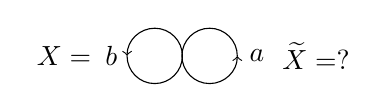
\begin{tikzpicture}
    \node at (-1.20,0) {$X=$};
    \draw [<-] (1,0) arc (360:0:10pt);
    \node at (1.25,0) {$a$};
    \draw [<-] (-0.40,0) arc (180:-180:10pt);
    \node at (-0.60,0) {$b$};
    \node at (2,0) {$\widetilde{X}=$?};
  \end{tikzpicture}

  $\widetilde{X}$ è rappresentato dal seguente grafo, con $\tilde{a}$ rappresentato dalle frecce orizzontali dirette verso destra (e $\tilde{a}^{-1}$ verso sinistra) e $\tilde{b}$ da quelle verticali verso l'alto (e $\tilde{b}^{-1}$ verso il basso):
  \begin{center}
    \begin{tikzpicture}
      \draw l-system [l-system={cayley, axiom=[A] [+A] [++A] [-A], step=1cm, order=3}];
      \node at (0.5,-0.15) {$\tilde{a}$};
      \node at (0.15,0.5) {$\tilde{b}$};
    \end{tikzpicture}
  \end{center}
  È un albero quadrivalente infinito. I segmenti orizzontali si proiettano su $a$, quelli verticali su $b$. Chi è il rivestimendo di $X$ associato ad $H=\langle a \rangle$? Cerchiamo un rivestimento $E \xrightarrow[]{p} X$ con $p_{\star}(\pi_1(E, \tilde{x}))=\langle a \rangle$. Il grafo è il seguente:
  \begin{center}
    \begin{tikzpicture}
      \draw l-system [l-system={cayley, axiom=[+A] [-A], step=1cm, order=3}];
      \draw [->] (0.7,0) arc (360:0:10pt);
      \node at (0.95,0) {$a$};
      \node at (-0.3,0) {$\tilde{x}_0$};
      \filldraw (0,0) circle (1pt);
    \end{tikzpicture}
  \end{center}
  Non è omogeneo: se $\varphi:E \rightarrow E$ è un omeomorfismo, $\varphi(\text{loop})=\text{loop} \implies \varphi(\tilde{x}_0)=\tilde{x}_0 \implies \text{Aut}(E)=\{1\}$. In effetti $\langle a \rangle$ è molto lontano dall'essere normale in $\pi_1(X, x)=\mathbb{Z} * \mathbb{Z}$.
  Se $N(a)$ è il sottogruppo normale generato da $a$ in $\pi_1(X)$, il rivestimento associato a $N$ come sarà fatto?
  $N$ normale $\implies$ il rivestimento associato $E \xrightarrow[]{p} X$ sarà regolare e $\text{Aut}(E)=\faktor{\pi_1(X, x)}{p_{\star}(\pi_1(E, \tilde{x}))}=\faktor{\mathbb{Z} * \mathbb{Z}}{N}=\langle a, b \mid a \rangle \overset{\psi}{\cong} \mathbb{Z}$,
  \begin{align*}
    \psi:\mathbb{Z}*\mathbb{Z} &\longrightarrow \mathbb{Z} \\
    a &\longmapsto 0 \\
    b &\longmapsto 1
  \end{align*}
  induce l'isomorfismo. Ecco $E$:
  \begin{center}
    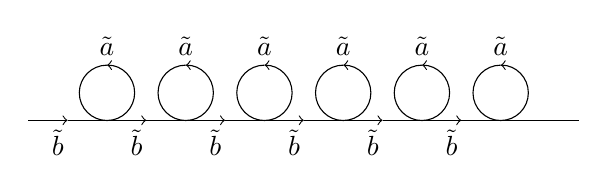
\begin{tikzpicture}
      \draw[->] (0,0) -- node[below, near end]{$\tilde{b}$} (0.5,0);
      \draw (0.5,0) -- (1,0);
      \draw [<-] (1,0.7) arc (450:90:10pt) node[above]{$\tilde{a}$};
      \draw[->] (1,0) -- node[below, near end]{$\tilde{b}$} (1.5,0);
      \draw (1.5,0) -- (2,0);
      \draw [<-] (2,0.7) arc (450:90:10pt) node[above]{$\tilde{a}$};
      \draw[->] (2,0) -- node[below, near end]{$\tilde{b}$} (2.5,0);
      \draw (2.5,0) -- (3,0);
      \draw [<-] (3,0.7) arc (450:90:10pt) node[above]{$\tilde{a}$};
      \draw[->] (3,0) -- node[below, near end]{$\tilde{b}$} (3.5,0);
      \draw (3.5,0) -- (4,0);
      \draw [<-] (4,0.7) arc (450:90:10pt) node[above]{$\tilde{a}$};
      \draw[->] (4,0) -- node[below, near end]{$\tilde{b}$} (4.5,0);
      \draw (4.5,0) -- (5,0);
      \draw [<-] (5,0.7) arc (450:90:10pt) node[above]{$\tilde{a}$};
      \draw[->] (5,0) -- node[below, near end]{$\tilde{b}$} (5.5,0);
      \draw (5.5,0) -- (6,0);
      \draw [<-] (6,0.7) arc (450:90:10pt) node[above]{$\tilde{a}$};
      \draw (6,0) -- (6.5,0);
      \draw (6.5,0) -- (7,0);
    \end{tikzpicture}
  \end{center}
\end{ex}
